% Lecture Template for ME3001-001-Tristan Hill - Spring 2017 - Fall 2017
% 
% Mechanical Engineering Analysis with MATLAB
%
% Introduction to Analysis

% Document settings
\documentclass[11pt]{article}
\usepackage[margin=1in]{geometry}
\usepackage[pdftex]{graphicx}
\usepackage{multirow}
\usepackage{setspace}
\usepackage{hyperref}
\usepackage{color,soul}
\usepackage{fancyvrb}
\usepackage{framed}
%\usepackage{wasysym}
\usepackage{multicol}
\usepackage{ amssymb }
\usepackage{amsmath}



\pagestyle{plain}
\setlength\parindent{0pt}
\hypersetup{
    bookmarks=true,         % show bookmarks bar?
    unicode=false,          % non-Latin characters in Acrobat’s bookmarks
    pdftoolbar=true,        % show Acrobat’s toolbar?
    pdfmenubar=true,        % show Acrobat’s menu?
    pdffitwindow=false,     % window fit to page when opened
    pdfstartview={FitH},    % fits the width of the page to the window
    pdftitle={My title},    % title
    pdfauthor={Author},     % author
    pdfsubject={Subject},   % subject of the document
    pdfcreator={Creator},   % creator of the document
    pdfproducer={Producer}, % producer of the document
    pdfkeywords={keyword1} {key2} {key3}, % list of keywords
    pdfnewwindow=true,      % links in new window
    colorlinks=true,       % false: boxed links; true: colored links
    linkcolor=red,          % color of internal links (change box color with linkbordercolor)
    citecolor=green,        % color of links to bibliography
    filecolor=magenta,      % color of file links
    urlcolor=blue           % color of external links
}

% assignment number 
\newcommand{\NUM}{1 } 
\newcommand{\VSpaceSize}{2mm} 
\newcommand{\HSpaceSize}{2mm} 

\newcommand{\Lagr}{\mathcal{L}}

\definecolor{mygray}{rgb}{.6, .6, .6}

\setulcolor{red} 
\setstcolor{green} 
\sethlcolor{mygray} 

\begin{document}

\textbf{ \LARGE ME 3050 Lecture - Dynamic Modeling and Controls} \vspace{3mm}\\
\textbf{ \hspace*{5mm}Tristan W. Hill - Tennessee Technological University - Spring 2020 } \vspace{3mm}\\


\textbf{ \LARGE Ch. 8 - System Response in the Time Domain} \\

\begin{itemize}


\item \textbf{ \LARGE (8.2) Time Response of 2$^{nd}$ Order Systems} \\

\begin{itemize}


\item \textbf{ \Large Now consider our mass-spring-damper system.}\\

			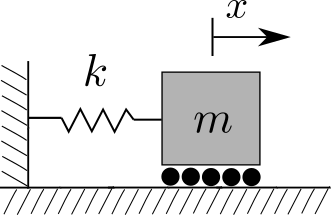
\includegraphics[scale=.5]{mass_spring_01.png} \\

\item \textbf{ \Large The EOM is:}\\

	\scalebox{1.5}{$m\ddot{x} +kx=0$\hspace{5mm}with\hspace{5mm}$ x(t=0)=x_0$, \hspace{5mm}and\hspace{5mm}$v(t=0)=v_0$} \\

\item \textbf{ \Large You have practiced solving for $x(t)$. Look at the solution. } \vspace{3mm}\\

	\scalebox{1.5}{$x(t)=\frac{v_0}{\omega_n}sin(\omega_nt)+x_0cos(w_nt) $\hspace{5mm}with\hspace{5mm} $\omega_n=\sqrt{\frac{k}{m}}$} \vspace{3mm}\\

\item \textbf{\large The solution is more commmonly used in the following form. The phase shift $\phi$ has been introduced. } \vspace{3mm}\\

	\scalebox{1.5}{$x(t)=Acos(\omega_nt-\phi)$\hspace{5mm}$A=\sqrt{x_0^2+[\frac{v_0}{\omega_n}]^2}$\hspace{5mm}$\phi=tan^{-1}(\frac{v_0}{x_0\omega_n})$} \\

\item \textbf{\large Or we could use sine instead}\vspace{3mm}\\

\scalebox{1.5}{$x(t)=Asin(\omega_nt+\phi)$\hspace{5mm}$A=\sqrt{x_0^2+[\frac{v_0}{\omega_n}]^2}$\hspace{5mm}$\phi=tan^{-1}(\frac{x(0)\omega_n}{v_0})$} \\


	\newpage
\item \textbf{ \Large Sketch the System Response in the time Domain.}


\includegraphics[scale=1]{lecture1_fig1.png} \\

\item \textbf{\large Is this a stable system? What does that even mean?}\\\\


\end{itemize}
		

	\newpage
\item \textbf{ \Large Now bring the damper back.}\\
\begin{multicols}{2}
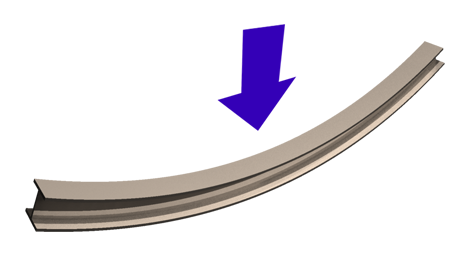
\includegraphics[scale=.40]{beam_bending_01.png} \\

\scalebox{1.5}{$m\ddot{x} +c\dot{x}+kx=0$} \\\\

%\[f(t) = \begin{cases} 
 %     0 & t < 0 \\
  %    F & t\geq 0 \\
 %  \end{cases}
%\]\\

\end{multicols}

\item \textbf{\large The trial solution method is shown.}\\\\

	\scalebox{1.5}{$m\ddot{x} +c\dot{x}+kx=0$ $ \implies$  $(mr^2+cr+k)Ae^{rt}=0$} \\\\

\item \textbf{\large You can see the Characteristic Equation becomes:}\\\\

	\scalebox{1.5}{$(mr^2+cr+k)=0$} \\

\item \textbf{\large Now you can solve for the roots. In system dynamics they are called $s_{1,2}$}\\\\

	\scalebox{1.5}{$r_{1,2}=s_{1,2}=\frac{-c\pm\sqrt{c^2-4mk}}{2m}=-\frac{c}{2m}\pm\sqrt{(\frac{c}{2m})^2-\frac{k}{m}}$} \\

\item \textbf{\large The roots of the system determine the nature of the behaviour.}\\\\

\scalebox{1.5}{$c^2-4mk=0$\hspace{5mm}and\hspace{5mm}$c=2\sqrt{mk}$} \\

\item \textbf{\large This value of c is called the \underline{critical damping value}.}\\\\


\scalebox{1.5}{if \hspace{5mm} $c<2\sqrt{mk}$\hspace{5mm}the system will oscillate}\vspace{5mm} \\
\scalebox{1.5}{if \hspace{5mm} $c\geq2\sqrt{mk}$\hspace{5mm}the system will NOT oscillate} \vspace{5mm}\\


\newpage
\item \textbf{\large Now we want to quatify \underline{how much} damping there is in the system.}\\\\

\textbf{\large The damping ratio $\zeta$ is the ratio of actual damping, c, to critical damping. }\\\\

\scalebox{1.5}{$\zeta=\frac{c}{2\sqrt{mk}}$} \\


\item \textbf{\large We can now re-write the roots with this new quantity.}\\\\

\scalebox{1.5}{$s_{1,2}=-\zeta\omega_n\pm\omega_n\sqrt{\zeta^2-1}=-\zeta\omega_n\pm j\omega_n\sqrt{1-\zeta^2}$}\\


\item \textbf{\large We define one more important new quantity, \underline{damped natural frequency}.}\\\\
	

\scalebox{1.5}{$\omega_d=\omega_n\sqrt{1-\zeta^2}$} \\\\

\item \textbf{\large We can now re-write the roots one more time.}\\\\

\scalebox{1.5}{$s_{1,2}=\zeta\omega_n\pm j\omega_d$}

\end{itemize}

\end{document}



